% Тут используется класс, установленный на сервере Papeeria. На случай, если
% текст понадобится редактировать где-то в другом месте, рядом лежит файл matmex-diploma-custom.cls
% который в момент своего создания был идентичен классу, установленному на сервере.
% Для того, чтобы им воспользоваться, замените matmex-diploma на matmex-diploma-custom
% Если вы работаете исключительно в Papeeria то мы настоятельно рекомендуем пользоваться
% классом matmex-diploma, поскольку он будет автоматически обновляться по мере внесения корректив
%

% По умолчанию используется шрифт 14 размера. Если нужен 12-й шрифт, уберите опцию [14pt]
\documentclass[14pt]{matmex-diploma}
%\documentclass[14pt]{matmex-diploma-custom}

\usepackage{ amssymb }
\usepackage[utf8]{inputenc}
\usepackage{babel}
\usepackage{amsthm}
\usepackage{algorithm}
\usepackage{multicol, multirow}

\usepackage{amsmath}
\usepackage{fancyvrb}
\usepackage{tikz}
\usepackage{pgfplots}
\usepackage{fontawesome}

\usetikzlibrary{automata, positioning, shapes,arrows}

\usepackage[caption=false]{subfig}
\usepackage{minted}
\usepackage{sidecap} 
\usepackage{fancyvrb}
\usepackage{wrapfig}
\usepackage{graphicx}
\usepackage{float}
\usepackage{color, colortbl}

\usepackage[noend]{algpseudocode}

\definecolor{green}{RGB}{34, 189, 65}

\theoremstyle{definition}
\newtheorem{definition}{Определение}[section]

\begin{document}
% Год, город, название университета и факультета предопределены,
% но можно и поменять.
% Если англоязычная титульная страница не нужна, то ее можно просто удалить.
\filltitle{ru}{
    chair              = {Математическое обеспечение и администрирование\\ информационных систем \\ Системное программирование},
    title              = {Поиск путей в графовых базах данных через тензорное произведение},
    % Здесь указывается тип работы. Возможные значения:
    %   coursework - Курсовая работа
    %   diploma - Диплом специалиста
    %   master - Диплом магистра
    %   bachelor - Диплом бакалавра
    type               = {coursework},
    position           = {студента},
    group              = 344,
    author             = {Илья Владимирович Эпельбаум},
    supervisorPosition = {к.\,ф.-м.\,н., доцент},
    supervisor         = {С.\,В. Григорьев },
    %reviewerPosition   = {ст. преп.},
    %reviewer           = {Привалов А.\,И.},
    %chairHeadPosition  = {д.\,ф.-м.\,н., профессор},
    %chairHead          = {Терехов А.\,Н.},
%   university         = {Санкт-Петербургский Государственный Университет},
%   faculty            = {Математико-механический факультет},
%   city               = {Санкт-Петербург},
%   year               = {2013}
}

\maketitle
\tableofcontents
% У введения нет номера главы
\section*{Введение}
Сегодня людям необходимо иметь доступ к большому объему информации. Для этого были придуманы базы данных. Разработано множество моделей построения баз данных. Например, часто используемой моделью является реляционная, где данные представлены в виде отношений. Однако данный тип не всегда представляется удобным в использовании, так как не обладает гибкостью во внесении изменений. В свою очередь, графовая модель данных обладает этим достоинством, что говорит о её конкурентоспособности. Впервые применение такой модели в базе данных предложена Михалисом Яннакакисом~\cite{firstGDB}. В ней информация представляется в виде вершин (сущности) и дуг (связи между сущностями). Примером графовой СУБД является Neo4j\footnote{Официальный сайт Neo4j: https://neo4j.com. Дата посещения: 16.05.2020.}.

Также возникает потребность в обработке информации. Например, осуществлять поиск путей в графовой базе данных. В основе графовой базы данных лежит граф, поэтому далее в рамках данной работы естественно отождествлять эти понятия и свести задачу поиска путей в такой базе данных к поиску путей в графе.

Имеется множество подходов к поиску путей в графе c ограничениями. Один из таких способов предоставляет теория формальных языков. А именно, пусть имеется помеченный граф, где метки взяты из некоторого алфавита. При таких допущениях наличие пути сразу же свидетельствует о наличии слова, полученного конкатенацией меток на дугах. Соответственно множество путей является множеством слов, то есть по определению оказывается языком. Теперь, чтобы ввести ограничения на эти пути, предлагается задать грамматику, которая будет описывать необходимый язык, то есть пути с необходимыми ограничениями. Таким образом алгоритм поиска путей должен выдавать только те пути, объединение меток которых является словом языка, порождаемого грамматикой. 

Данный подход применяется в следующих областях: статический анализ кода~\cite{Stat}, биоинформатика~\cite{Bio}, анализ RDF файлов~\cite{RDF}.

Существует множество алгоритмов, решающих данную задачу. Однако авторы статьи \cite{oper_matrix}, взяв существующие алгоритмы, показали, что каждый из них может быть успешно применен в промышленных продуктах лишь при определенных условиях на входные данные. Но при этом в общем виде требуют больших вычислительных ресурсов, поэтому успешное использование их в настоящее время не представляется возможным. Вместе с этим, в недавнем исследовании, проведенном авторами статьи \cite{mishin}, было продемонстрировано, что линейная алгебра является одним из путей к высокопроизводительным алгоритмам в данной области. Вследствие этого лабораторией языковых инструментов JetBrains ведутся разработки новых более эффективных методов, использующих этот подход. Результатом такой деятельности стал алгоритм, основанный на тензорном произведении. Соответственно, возникает потребность в сравнении этого результата с конкурирующими алгоритмами.

\section{Постановка задачи}
Целью данной работы является сравнение алгоритма, основанного на тензорном произведении, и алгоритма, основанного на матричном умножении. Для достижения цели были поставлены приведённые ниже задачи.

\begin{enumerate}
    \item Реализовать алгоритм поиска путей через тензорное произведение.
    
    \item Внедрить реализацию в СУБД RedisGraph.
    
    \item Произвести экспериментальное исследование производительности реализации. Для демонстрации затраченного времени для работы реализованного алгоритма над исходными данными использовать набор данных \footnote{Репозиторий набора данных: https://github.com/JetBrains-Research/CFPQ\_Data . Дата посещения: 16.05.2020.}.
\end{enumerate}

\section{Обзор}
Приведем определения понятий, которые используются в работе.
\subsection{Базовые определения}
Следующее определение описывает структуру представления грамматики, которую использует алгоритм, основанный на тензоронм произведении.
\theoremstyle{definition}
\begin{definition}
Рекурсивный автомат \cite{rec} над конечным алфавитом $\Sigma$ есть набор $(M,m,\{C_i\}_{i \in M})$, где 

\begin{itemize}
    \item $M$ конечное множество меток,
    \item $m \in M$ начальная метка,
    \item $ \{C_i\}_{i \in M} $ множество \textit{конечных автоматов},
          где $C_i=(\Sigma \cup M, Q_i,q_i^0,F_i,\delta_i)$:
    \begin{itemize}
        \item $\Sigma \cup M$ множество символов, $\Sigma \cap M = \emptyset$,
        \item $Q_i$ конечное множество состояний,
              где $Q_i \cap Q_j = \emptyset, \forall i \neq j$,
        \item $q_i^0$ начальное состояние $C_i$,
        \item $F_i$ множество финальных состояний $C_i$, где $F_i \subseteq Q_i$,
        \item $\delta_i$ функция переходов $C_i$,
              где $\delta_i: Q_i \times (\Sigma \cup M)
              \to Q_i$.
    \end{itemize}
\end{itemize}
\end{definition}

\begin{definition}
Пусть G = $\langle \Sigma, $N$, $P$, $S$ \rangle$ констекстно-свободная грамматика, тогда G находится в \textbf{ослабленной нормальной форме Хомского} (ОНФХ), если содержит только правила вида:
\begin{itemize}
    \item $A \rightarrow BC$, где $A$, $B$, $C \in N$
    \item $A \rightarrow a$, где $A \in N$, $a \in \Sigma$
    \item $A \rightarrow \varepsilon$, где $A \in N$
\end{itemize}
\end{definition}

Определение ОНФХ отличается от нормальной формы Хомского наличием правил вида $A \rightarrow \varepsilon$, где А --- любой нетерминал, то есть А не обязательно является стартовым, а также допущением использовать стартовый нетерминал в правых частях правил.

\subsection{Алгоритм, основанный на матричном умножении}

В настоящий момент существует два алгоритма для КС запросов, использующих линейную алгебру. Первый предложен аспирантом кафедры системного программирования, Рустамом Азимовым \cite{alg_matrix}. Имеет сложность $O(n^{2}|N|^{2}|P|(MM(n)))$, где $|P|$ --- количество правил грамматики, $|N|$ --- мощность множества нетерминалов, MM(n) --- сложность умножения квадратных матриц размера n. Основан на обычном произведении матриц, что позволяет достичь хорошей производительности. Однако он требует, чтобы грамматика находилась в ослабленной нормальной форме Хомского, что приводит к её разрастанию и, как следствие, отрицательно сказывается на производительности и потребляемой памяти. В борьбе с этим, был разработан другой алгоритм. Он основан на тензорном произведении.

\subsection{Алгоритм, основанный на тензорном произведении}

На листинге 1 приведен алгоритм, основанный на тензорном произведении. На вход алгоритм принимает ориентированный помеченный граф $\mathcal{G} = \langle V, E, L \rangle$ и грамматику G.

Сначала, используя подход, описанный в статье \cite{rec}, строится рекурсивный автомат для G. Далее пусть $M_{1}$ --- матрица смежности рекурсивного автомата, а $M_{2}$ --- матрица смежности $\mathcal{G}$. На первом шаге вычисляется тензорное произведение $M_{1}$ и $M_{2}$, тем самым пересекая два автомата (граф и рекурсивный автомат). После чего результат транзитивно замыкается. Следующим шагом, обходя матрицу транзитивного замыкания, проверяется наличие ребра, и принадлежность начальной и конечной вершин стартовому и конечному состоянию рекурсивного автомата, для этого на листинге 2 приведены вспомогательные функции. При выполнении условия алгоритм добавляет нетерминал/нетерминалы, соответствующие стартовому и конечному состоянию автомата, в ячейку $M_{2}$. Данные шаги алгоритма повторяются пока матрица $M_{2}$ изменяется. За каждую итерацию $i$ получаются пути, выводимые из грамматики за $i$ шагов. Результатом работы алгоритма является матрица $M_{2}$

\begin{algorithm}[H]
\floatname{algorithm}{Listing}
\begin{algorithmic}[1]
\caption{Алгоритм}
\label{tensor:cfpq}
\Function{contextFreePathQuerying}{G, $\mathcal{G}$}
    % Input data preparation
    \State{$R \gets$ Рекурсивный автомат для $G$}
    \State{$M_1 \gets$ Матрица смежности для $R$}
    \State{$M_2 \gets$ Матрица смежности для $\mathcal{G}$}
    % Eps-transition handling for graph
    \For{$s \in 0..dim(M_1)-1$}
        \For{$i \in 0..dim(M_2)-1$}
            \State{$M_2[i,i] \gets M_2[i,i] \cup \textit{getNonterminals}(R,s,s)$}
        \EndFor
    \EndFor
    \While{Матрица $M_2$ изменяется}
        \State{$M_3 \gets M_1 \otimes M_2$}
        \Comment{Вычисление тензорного произведения}
        \State{$C_3 \gets \textit{transitiveClosure}(M_3)$}
        \State{$n \gets$ dim($M_3)$}
        % Add non-terminals (possibly new)
        \For{$i \in 0..n-1$}
           \For{$j \in 0..n-1$}
                \If{$C_3[i,j]$}
                    \State{$s, f \gets \textit{getStates}(C_3,i,j)$}
                    \If{$\textit{getNonterminals}(R,s,f) \neq \emptyset$}
                        \State{$x, y \gets \textit{getCoordinates}(C_3,i,j)$}
                        \State{$M_2[x,y] \gets M_2[x,y] \cup \textit{getNonterminals}(R,s,f)$}
                    \EndIf
                \EndIf
           \EndFor
        \EndFor
    \EndWhile
\State \Return $M_2$
\EndFunction
\end{algorithmic}
\end{algorithm}

\begin{algorithm}[H]
\floatname{algorithm}{Listing}
\begin{algorithmic}[1]
\caption{Вспомогательные функции}
\label{tensor:cfpq:help}
\Function{getStates}{$M_1, i, j$}
    \State{$r \gets dim(M_1)$}
    \State \Return{$\left\lfloor{i / r}\right\rfloor, \left\lfloor{j / r}\right\rfloor$}
\EndFunction
\Function{getCoordinates}{$M_2, i, j$}
    \State{$n \gets dim(M_2)$}
    \State \Return{$i \bmod n, j \bmod n$}
\EndFunction
\end{algorithmic}
\end{algorithm}

Данный алгоритм использует рекурсивный автомат, что полностью избавляет от необходимости преобразовывать грамматику, а также полностью основан на линейно алгебре. Однако в процессе работы, а именно в результате тензорного произведения, возникают матрицы больших размеров. Например, если тензорно перемножить одну матрицу размером $m \times p$ и вторую матрицу $n \times q$, то в результате получается матрица $mn \times pq$, что может отрицательно сказаться на производительности.
\subsection{Используемые технологии}
Рассмотрим технологии, которые используются для реализации и внедрения алгоритма, основанного на тензорном произведении.
\subsubsection{Библиотека SuiteSparse}

Для реализации был выбрана библиотека SuiteSparse\footnote{Сайт проекта: http://faculty.cse.tamu.edu/davis/suitesparse.html. Дата посещения: 16.05.2020.}. SuiteSparse является реализацией API GraphBlas. Обладает широким спектром возможностей \cite{MathInGB} для реализаций алгоритмов, которые подобны изложенным выше, так как создавался для произведения операций над графами средствами линейной алгебры. Например, предоставляет возможность определять новые полукольца с операциями, которые также можно определять. В частности имеет встроенное тензорное произведение над булевым полукольцом. Также позволяет хранить матрицы, учитывая свойство разреженности, что необходимо для эфективной реализации алгоритма, основанного на тензорном произведении.

\subsubsection{Графовая база данных RedisGraph}

Для внедрения реализации была выбрана СУБД RedisGraph\footnote{Репозиторий проекта RedisGraph: https://github.com/RedisGraph/RedisGraph. Дата посещения: 16.05.2020.}. СУБД с открытым исходным кодом, что предоставляет возможность полноценно внедрить реализацию алгоритма. RedisGraph использует стандарт GraphBlas для выполнения операций над графами, что упрощает интеграцию алгоритма. Одним из главных факторов выбора является быстродействие работы СУБД, а как показано в статье \cite{DBLP}, RedisGraph является конкурентноспособной СУБД по данному направлению. Изложенные аргументы подтверждают правильность выбора платформы для выполнения поставленной цели.


\section{Реализация и интеграция}

\subsection{Подход к реализации}

Для реализации поставленной задачи был применен следующий подход. Вместо обычной матрицы смежности графа для каждой метки заводится булева матрица смежности графа, то есть в матрице на месте $(i;j)$ стоит 1, если в графе из вершины $i$ в вершину $j$ есть дуга с соответствующей меткой. Продемонстрируем на примере.

\bigskip

\begin{minipage}[m]{0.2\linewidth}

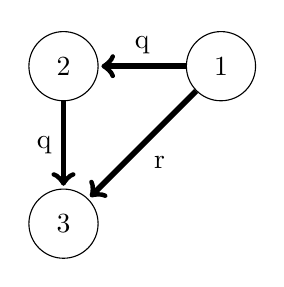
\begin{tikzpicture}[shorten >=1pt,node distance=2cm,on grid,auto]
   \node[state] (x) {1};
   \node[state] (b) [left=of x] {2};
   \node[state] (e) [below=of b] {3};
   \path[->]
    (x) edge[line width=2pt] node[above] {q} (b)
    (x) edge[line width=2pt] node        {r} (e)
    (b) edge[line width=2pt] node[left]  {q} (e);
\end{tikzpicture}

\end{minipage}
$\Rightarrow$\hfill
\begin{minipage}[m]{0.12\linewidth}
$\begin{bmatrix} 
0 & q & r \\
0 & 0 & q \\
0 & 0 & 0
\end{bmatrix}
$
\end{minipage}
$\Rightarrow$\hfill
\begin{minipage}[m]{0.5\linewidth}

$r: \begin{bmatrix} 0 & 0 & 1 \\ 0 & 0 & 0 \\ 0 & 0 & 0 \end{bmatrix}, q: \begin{bmatrix} 0 & 1 & 0 \\ 0 & 0 & 1 \\ 0 & 0 & 0 \end{bmatrix}$

\end{minipage}

\bigskip

В таком случае тензорное произведение вычисляется в булевом полукольце. А именно, вычисляется тензорное произведение булевых матриц смежности, которые соответствуют одним меткам, и результаты суммируются. 

\subsection{Архитектура}

В ходе работы над реализацией и интеграции алгоритма в RedisGraph были реализованы модули, указанные на рис. 1 синим цветом. Для их разработки использовался язык программирования C, так как исходный код RedisGraph написан на данном языке.

\begin{figure}[h]
\begin{center}
     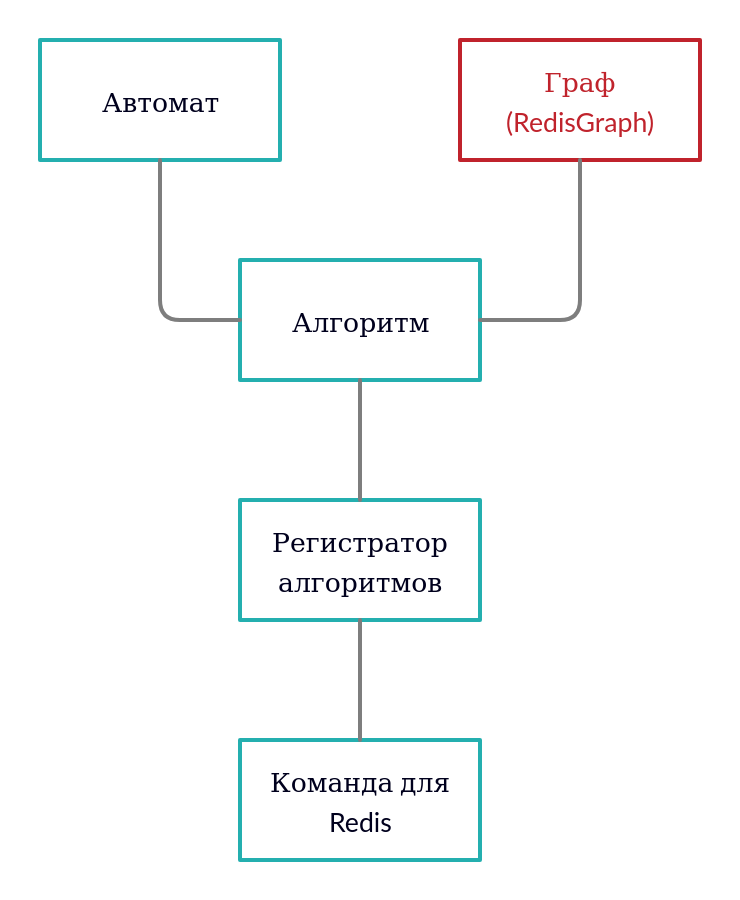
\includegraphics[height=10cm]{diagram.jpg}
     \caption{Модули}
\end{center}
\end{figure}

Модуль "Автомат" представляет структуру данных, использующую матрицы из библиотеки SuiteSparse, для хранения рекурсивного автомата. Матрица смежности представлена способом, описанным в разделе 3.1. Данная структура содержит только один метод для загрузки автомата из файла.

Модуль "Алгоритм" является реализацией алгоритма, основанного на тензорном произведении. Реализация принимает на вход граф из RedisGraph и экземпляр структуры данных рекурсивного автомата. Структура хранения графа в RedisGraph соответствует подходу, описанному в разделе 3.1. Поэтому для вычисления тензорного произведения матриц над булевым полукольцом используется встроенная функция библиотеки SuiteSparse.

Модуль "Регистратор алгоритмов" представляет структуру данных для хранения реализаций алгоритмов, использующих граф и рекурсивный автомат. Добавление алгоритма для последующего запуска в redis-server является обязательным.

Модуль "Команда для Redis" является реализацией команды для redis-server. Команда принимает 3 обязательных аргумента: название алгоритма, содержащееся в регистраторе алгоритмов, название графа из загруженных в RedisGraph и путь до автомата. При запуске команды происходит создание структуры данных рекурсивного автомата и его загрузка, после чего происходит запуск алгоритма.


\section{Эксперименты}

Для постановки экспериментов над реализацией был использован ПК с операционной системой Ubuntu 18.04 и конфигурацией: Intel(R) Core(TM) i7-4790 CPU @ 3.60GHz CPU, DDR4 32 Gb RAM. Сравнения производились с реализацией алгоритма, основанного на матричном умножении, использующая тот же набор технологий и ПК для проведения экспериментов. 

В качестве набора данных \footnote{Репозиторий набора данных: https://github.com/JetBrains-Research/CFPQ\_Data . Дата посещения: 16.05.2020.} были взяты графы следующих классов:
\begin{itemize}
    \item Worstcase --- теоретически наихудшая ситуация.
    \item FullGraph --- наихудшая ситуация для разреженных матриц.
    \item RDF --- реальные данные.
\end{itemize}

В ходе проведения экспериментов бралась выборка из 10 результатов над каждым классом. В итоге были получены следующие результаты.

\begin{figure}[h]
\begin{center}
     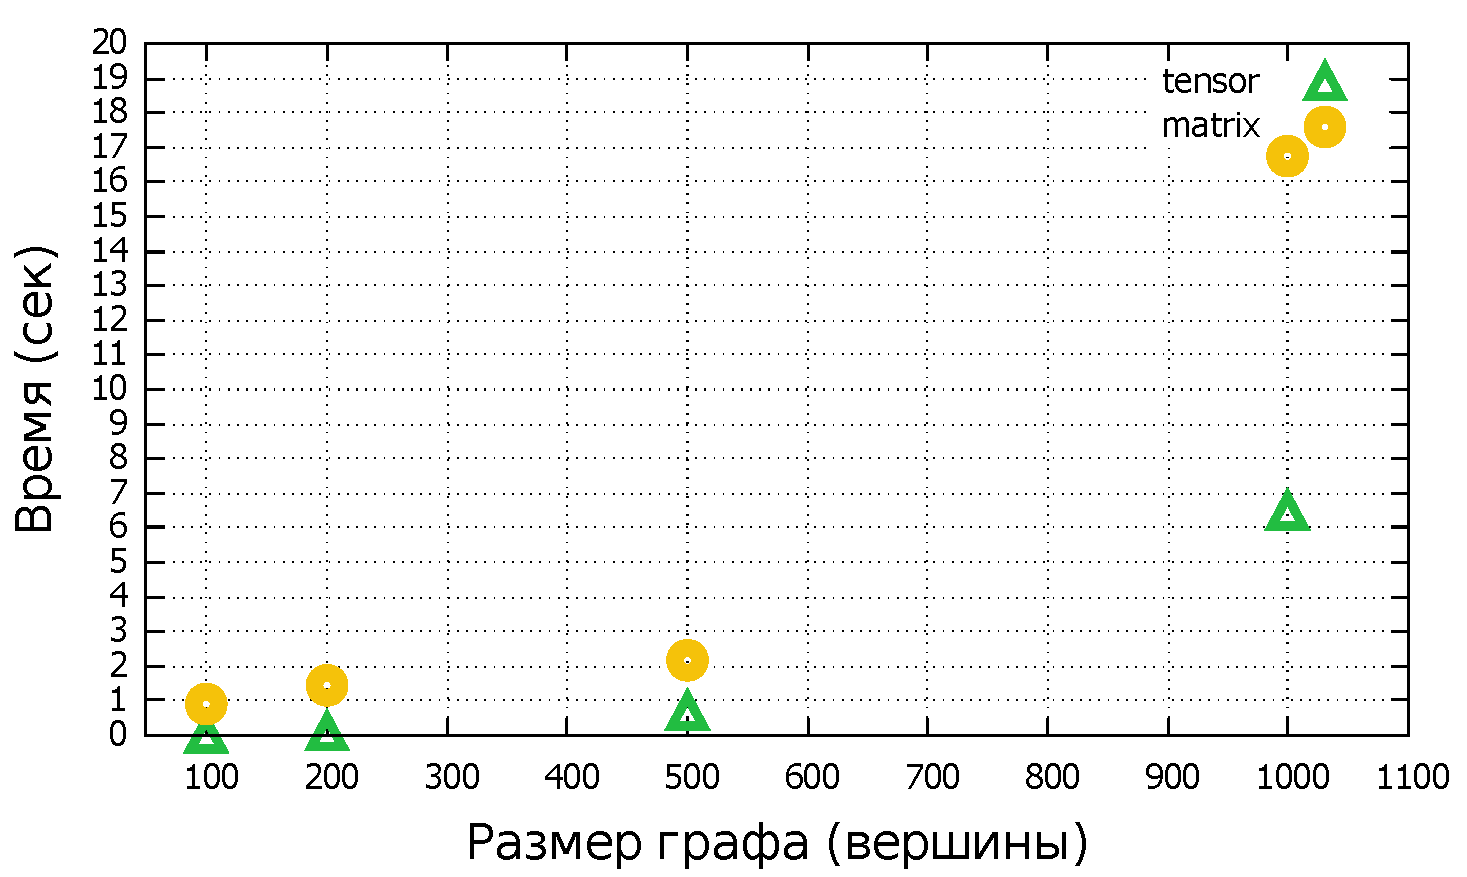
\includegraphics[width=10cm]{fullgraph.pdf}
     \caption{FullGraph}
\end{center}
\end{figure}
\begin{figure}[h]
\begin{center}
    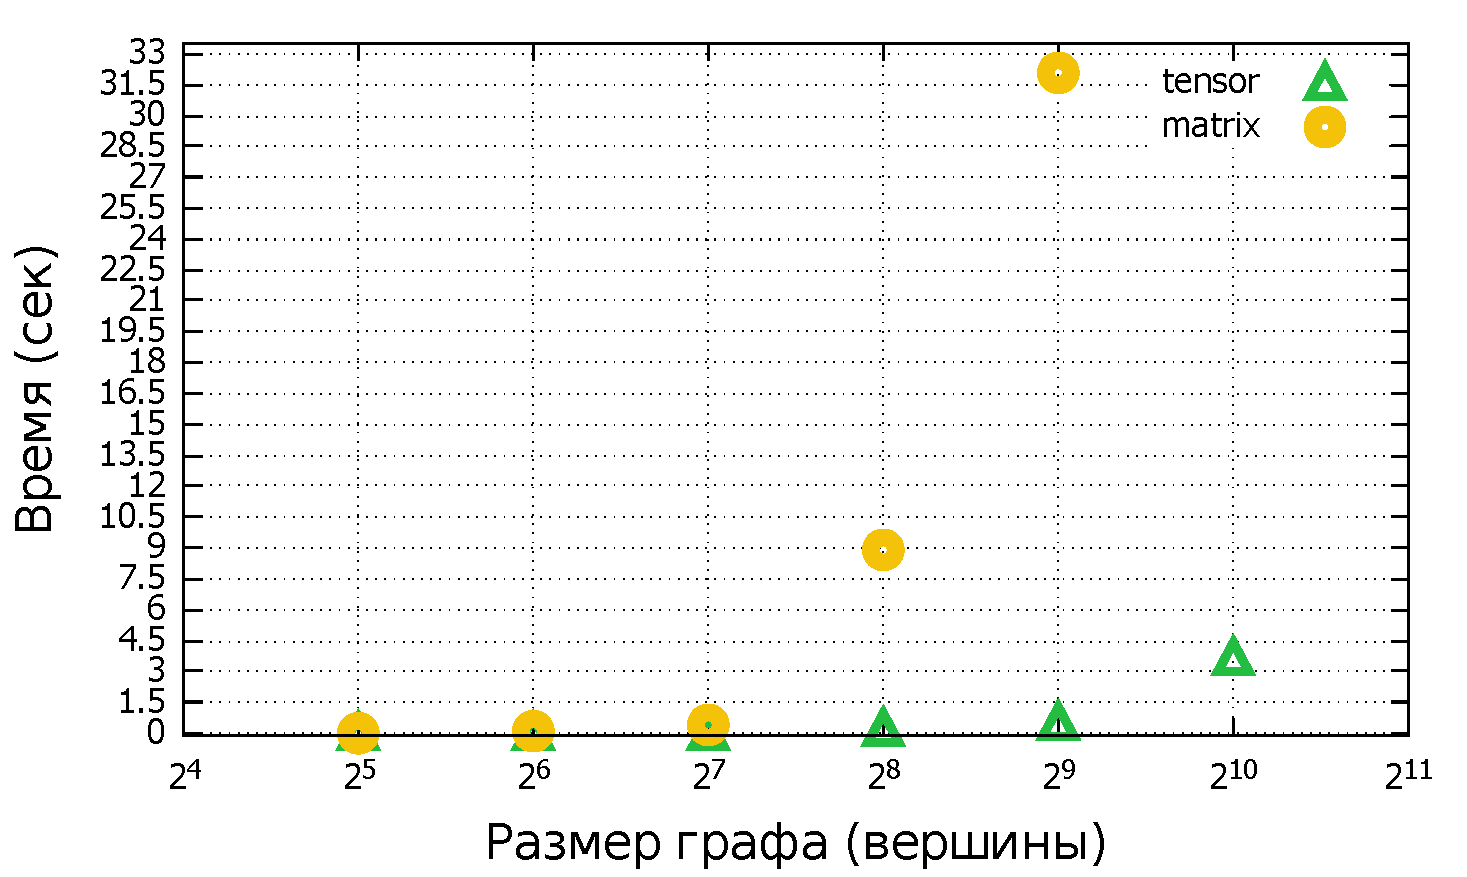
\includegraphics[width=10cm]{worstcase.pdf}
     \caption{Worstcase}
\end{center}
\end{figure}

На рис. 2 и рис. 3 представлены графики результатов замеров на классах FullGraph и Worstcase соответственно. Показатели алгоритма, основанного на тензорном произведении, демонстрируют превосходство над результатами алгоритма, предложенного Рустамом Азимовым, более чем в 50 раз и в 2 раза соответственно. Показатель для доверительного интервала --- $\pm \Delta = \pm 0,06$.

\begin{table}[h]
\begin{center}
\begin{tabular}{||c|c|c|c|c||}
        \hline
        \hline
             Граф & V & E & Tensor & Matrix \\
             \hline
             \hline
             \rowcolor{green}
             pathways & 6238 & 37196 & 0.008 & 0.009\\
             \hline
             go & 272770 & 1068622 & 1.744 & 0.604 \\
             \hline
             \rowcolor{green}
             atom-primitive & 291 & 685 & 0.011 & 0.016 \\
             \hline
             eclass\_514en & 239111 & 1047454 & 0.329 & 0.067 \\
             \hline
             \rowcolor{green}
             foaf & 256 & 815 & 0.001 & 0.002 \\
             \hline
             \rowcolor{green}
             funding & 778 & 1480 & 0.005 & 0.006 \\
             \hline
             go-hierarchy & 45007 & 1960436 & 0.179 & 0.091 \\
             \hline
             \rowcolor{green}
             bio-mesure & 341 & 711 & 0.010 & 0.016 \\
             \hline
             \rowcolor{green}
             pizza & 671 & 2604 & 0.026 & 0.030 \\
             \hline
             enzyme & 48815 & 219390 & 0.157 & 0.018 \\
             \hline
             \hline
        \end{tabular}
\end{center}
\caption{RDF}
\end{table}

В таблице 1 собраны результаты на реальных данных. Положительные показатели наблюдаются только на графах, отмеченных зеленым цветом, а именно: pathways, atom-primitive, foaf, pizza, funding, bio-mesure. Показатель для доверительного интервала --- $\pm \Delta = \pm 0,06$.

Таким образом из приведенных результатов экспериментов можно сделать следующие выводы.
\begin{itemize}
    \item Положительные результаты для RDF наблюдаются только на маленьких графах. Однако стоит заметить, что сравнения производились с реализацией, которая улучшалась в течение нескольких лет, а реализация алгоритма, представленная в работе, является единственной.
    \item Показатели на синтетических данных говорят о некотором потенциале нового алгоритма.
\end{itemize}

Приведенные выводы формируют некоторую картину производительности алгоритма в сравнении с алгоритмом, основанным на матричном умножении. Вследствие её можно сделать вывод о необходимости улучшения реализации для получения лучших результатов.

% У заключения нет номера главы
\section*{Заключение}
В рамках курсовой работы были выполнены следующие задачи:
\begin{enumerate}
    \item Реализован\footnote{Реализация: https://github.com/IlyaEp/RedisGraph/tree/IlyaEp\_tensor. Дата посещения: 16.05.2020.} алгоритм, основанный на тензорном произведении
        \item Реализация интегрирована в СУБД RedisGraph
        \item Произведены экспериментальные исследования производительности реализации на наборах данных:
        \begin{itemize}
            \item WorstCase
            \item FullGraph
            \item RDF
        \end{itemize}
\end{enumerate}
Также результаты работы изложены в статье "Context-Free Path Querying by Kronecker Product". Статья принята на конференцию ADBIS 2020.
В качестве дальнейших исследований предлагается следующее.
\begin{itemize}
    \item Произвести улучшение реализации алгоритма и сравнить новые результаты с существующими. Улучшения, например, могут состоять в использовании других методов библиотеки SuiteSparse для обновления графа и транзитивного замыкания.
    \item Реализовать восстановление путей и провести эксперименты для сравнения показателей с результатами алгоритма, основанного на матричном умножении, учитывая тот факт, что рассмотренный в работе алгоритм обладает возможностью восстанавливать все пути.
\end{itemize}

Работа проводилась в лаборатории языковых инструментов JetBrains-Research. Автор выражает благодарность сотрудникам лаборатории за всестороннюю помощь, а также за предоставленное оборудование для проведения экспериментов.

\setmonofont[Mapping=tex-text]{CMU Typewriter Text}
\bibliographystyle{ugost2008ls}
\bibliography{diploma.bib}
\end{document}
